\documentclass[runningheads]{llncs}
\usepackage[utf8]{inputenc}
\usepackage{graphicx}
\usepackage{amsmath}
\usepackage{amsmath,amssymb,todonotes,xspace}
\usepackage{minted}
\usepackage{url}
\usepackage[hidelinks]{hyperref}           
\usepackage[style=numeric-comp, sorting=none, backend=biber, url=true]{biblatex}

\def\UrlBreaks{\do\/\do-}


\addbibresource{refs.bib}


\newcommand*{\CC}{\ensuremath{\mathcal{C}}\xspace}
\newcommand*{\DD}{\ensuremath{\mathcal{D}}\xspace}
\newcommand*{\ordCC}{\ensuremath{(\mathcal{C}, <_c)}\xspace}
\newcommand*{\chrs}{\texttt{chars}}
\newcommand*{\mro}{\texttt{MRO}}
\newcommand*{\natz}{\ensuremath{\mathbb{N}_0}}
\newcommand*{\cl}{\texttt{c3linearization}}
\newcommand*{\rem}{\texttt{remove}}
\newcommand*{\h}{\texttt{head}}
\newcommand*{\mer}{\texttt{merge}}
\newcommand*{\oneToN}{\ensuremath{[\![1,n]\!]}\xspace}

\title{Specification and Verification of C3 linearization algorithm}
\author{
  Miguel Flor \and Mário Pereira \and António Ravara
}
\authorrunning{M. Flor et al.}
\institute{
  NOVA LINCS, Nova School of Science and Technology \\
  \email{m.flor@campus.fct.unl.pt}, \email{\{mjp.pereira, aravara\}@fct.unl.pt}
}

\begin{document}
\maketitle

\begin{abstract}
Multiple inheritance is common in modern programming languages,
 and the C3 linearization algorithm is widely adopted to ensure a consistent and intuitive method resolution order (MRO). Despite its common use, particularly in Python, the algorithm is non-trivial, and rigorous formal specification and verification remain necessary.
In this paper, we present a mathematical formalization of the C3 algorithm and initiate its verification using OCaml, Why3, and Cameleer. Our work proves the termination and partial verification of the core components of the algorithm.
While complete verification of the linearization process is ongoing, our contributions represent an essential step toward a complete proof of C3's verification.

     
\end{abstract}
\section{Introduction}
The development of large software systems often requires object-oriented programming languages that support multiple inheritance and provide a predictable method resolution order (MRO). 
 That's why the C3 linearization algorithm is used in many programming languages Python 2.3\autocite{Python23Method}, Perl\autocite{MroMethodResolution}, Solidity\autocite{LanguageInfluencesSolidity}, and many others.
 Exactly because of its widespread use, there is a need for an implementation that is verified, in this paper the verification is done in OCaml using Why3 and Cameleer.

\subsection{Why C3?}
C3 algorithm is widely used for producing a consistent and predictable MRO when conflicts arise in multiple inheritance scenarios.
The algorithm uses three core properties to ensure that the MRO is consistent (these properties are explained in section~\ref{subsec:C3Linearization}):
\begin{itemize}
    \item Extended Precedence Graph (EPG)
    \item Local Precedence Order (LPO)
    \item Monotonicity
\end{itemize}
To understand the algorithm consider the class hierarchy in Fig.~\ref{fig:DiamondProblem}, where class $A$ inherits from both $B$ and $C$. The C3 algorithm resolves the conflict ensuring that the MRO respects the order of inheritance (reading from left to right), resulting in an MRO of $(A, B, C, D)$.

\subsection{Contributions}
To reach the goal of a verified implementation of the C3 linearization algorithm, we present the following contributions:
\begin{itemize}
    \item A mathematical formal specification of the C3 linearization algorithm, which includes the properties that the algorithm must satisfy.
    \item An Ocaml implementation of the C3 linearization algorithm.
    \item A partial verification of the implementation using Why3 and Cameleer, demonstrating essential correctness properties and termination.
\end{itemize}
Both the formal specification and the implementation are available in the repository\autocite{MiguelflorC3_ocaml_verified}.
\section{Background}

We will first examine how multiple inheritance affects MRO algorithms, then examine the principles of the C3 linearization algorithm, followed by a brief overview of cameleer.

\subsection{Influence of Multiple Inheritance on MRO Algorithms}
MRO is a linear extension of some class hierarchy
 that induces a total order on the classes in the hierarchy\autocite{hivertControllingC3Super2024}.

\begin{figure}[htbp]
  \centering
  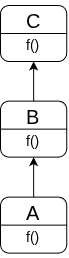
\includegraphics[width=0.06\textwidth]{images/SimpleDiagram.png}
  \caption{Simple graph}
  \label{fig:simpleDiagram}
\end{figure}

For the example above (Fig.~\ref{fig:simpleDiagram}) a logical MRO could be $(A, B, C)$, this means that when the function f is executed from the class $A$ the implementation of $A$ will be prioritized over $B$, and the implementation of $B$ will be prioritized over $C$.\\
However, the MRO of a class hierarchy is not always that straightforward, and conflicts can start to arise when we introduce multiple inheritance.
To demonstrate this, consider the following example, that represents a known problem called the diamond problem\autocite{mondayezeStudiesObjectorientedProgramming2021}.
\begin{figure}[htbp]
  \centering
  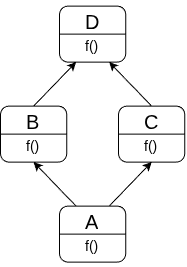
\includegraphics[width=0.15\textwidth]{images/DiamondProblem.png}
  \caption{Diamond problem graph}
  \label{fig:DiamondProblem}
\end{figure}

In this example (Fig.~\ref{fig:DiamondProblem}), a conflict emerges when determining the MRO of class $A$, since $A$ inherits from both $B$ and $C$. This raises the question: Which implementation, $B$'s or $C$'s, does $A$ inherit from? 
This is where the C3 linearization algorithm comes into play, as it provides a consistent and predictable way to resolve this conflict, the algorithm says that we need to prioritize $B$ over $C$, because $B$ comes first in the class hierarchy, and therefore the MRO of $A$ will be $(A, B, C, D)$.

\subsection{C3 Linearization Algorithm}
\label{subsec:C3Linearization}
The C3 algorithm produces an MRO that is consistent with EPG, LPO, and monotonicity\autocite{barrettMonotonicSuperclassLinearization1996} (all of these properties are formally defined in section\ref{subsec:PropertiesformalSpec}).

\subsubsection{EPG}
To understand the EPG, consider the following graph (Fig.~\ref{fig:C3Diagram}). For this graph instead of ordering the classes from left to right,
 they are arranged by the weights of the directed edges, from smallest to largest.

\begin{figure}[htbp]
  \centering
  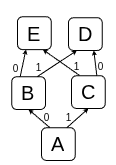
\includegraphics[width=0.15\textwidth]{images/NoneEPG.png}
  \caption{Inconsistent EPG}
  \label{fig:C3Diagram}
\end{figure}

This graph is inconsistent with the EPG, as the parent classes of $B$ and $C$ are ordered differently. A valid class hierarchy requires that for each class, the parent classes are ordered in the same way.
\subsubsection{LPO}
Consider the graph in Fig. \ref{fig:DiamondProblem}. An MRO that is consistent needs to respect the priority of the classes locally at each inheritance point; therefore, for this case, it cannot be $(A, C, B, D)$.
\subsubsection{Monotonicity}
If an MRO algorithm is consistency with monotonicity, it means that if a new class is added to the hierarchy the order of the previous MRO is preserved.

\subsection{Cameleer and Why3}
Cameleer\autocite{pereiraCameleerDeductiveVerification2021} is an automated tool for deductive verification in OCaml. It uses comments written in GOSPEL\autocite{chargueraudGOSPELProvidingOCaml2019} (Generic OCaml Specification Language) to specify the properties of functions, and then leverages Why3\autocite{filliatreWhy3WherePrograms2013a} to verify these properties.\\
With GOSPEL, we can write pre-conditions, post-conditions, invariants, and variants using comments that start with a @ and are attached to a specific OCaml function. Take the OCaml function below as an example:
\inputminted[fontsize=\small,linenos,xleftmargin=20pt]{ocaml}{../filter_heads/filter_heads.ml}
In the function \texttt{filter\_heads} takes a list of lists as argument and returns a list of the heads of each sublist, the GOSPEL comments two post-conditions and a variant.
The first post-condition (lines 7 and 8) states that for every element \( y \) in the result list \( r \), exists a sublist \( x \) in the input list \( l \) such that the head of \( x \) is equal to \( y \).
The second post-condition (lines 9) states that for every sublist \( x \) in the input list \( l \), the head of \( x \) is in the result list \( r \).
The variant (line 10) ensures the termination of the function by stating that the input list \( l \) is decreasing in size with each recursive call.\\
To run the verification, we can use the command \texttt{cameleer <file name>.ml}, which will open the Why3 IDE, like the one in Fig.\ref{fig:Why3FilterHeads}.

\begin{figure}[htbp]
  \centering
  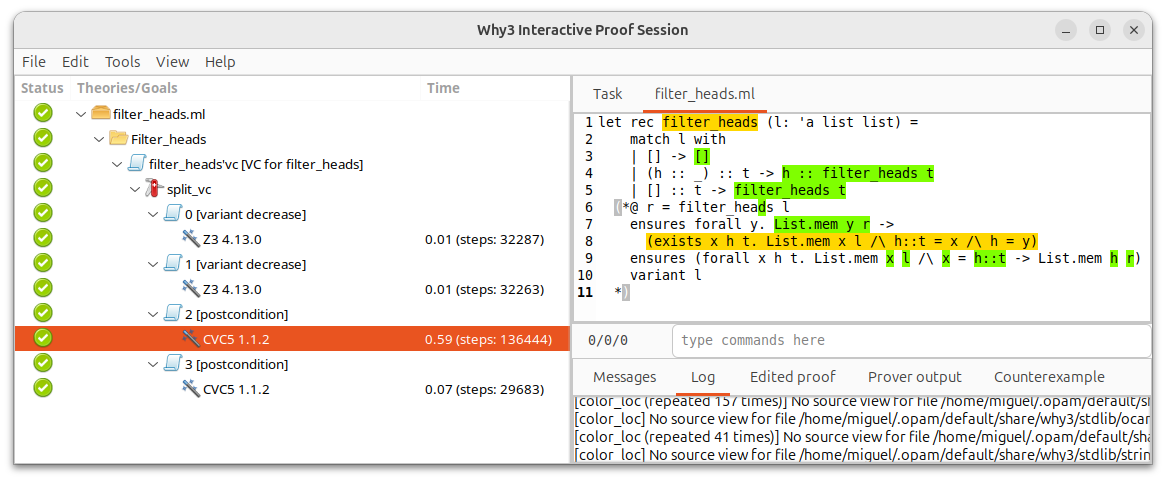
\includegraphics[width=1\textwidth]{images/Why3FilterHeads.png}
  \caption{\texttt{filter\_heads.ml} in Why3 IDE}
  \label{fig:Why3FilterHeads}
\end{figure}
As demonstrated by the green checkmark on the left side of the screen, the proof has been successfully verified. 
In the IDE, we proved these goals using provers, for our work we used three main provers,
 Alt-Ergo 2.6.0\autocite{sasAltErgoSMTSolver}, Z3 4.13.0\autocite{Z3ProverZ32025}, and CVC5 1.1.2\autocite{Cvc5} and for each goal, we can select which prover to use. To automate the proof Why3 provides a list of proof strategies including \texttt{Split\_vc}, \texttt{Auto\_level\_0}, \texttt{Auto\_level\_1}, 
\texttt{Auto\_level\_2}, and \texttt{Auto\_level\_3}. We also have commands to assist in the proof process, these commands are used to manipulate terms and hypotheses. All the commands and strategies are documented in Why3 documentation \autocite{12TechnicalInformations}.
Below is a list of commands that we utilized in our work:
\begin{itemize}
  \item \texttt{instantiate} 
  \item \texttt{induction\_arg\_ty\_lex}
  \item \texttt{intros} 
  \item \texttt{destruct}
  \item \texttt{destruct\_term}
  \item \texttt{unfold}
  \item \texttt{split\_vc}
  \item \texttt{inline\_goal}
\end{itemize}

\section{Formal Specification of C3 Linearization Algorithm}


\subsection{Ingredients}

Let \CC be a finite set of symbols, ranged over by \( C_0, C_1, \ldots, C_n \), possibly primed, which we refer to as \emph{classes}, and let \ordCC be an ordered set of classes. %\\

Consider $\mathcal P \subseteq \ordCC$ and $\DD \subseteq \CC \times \wp{(\mathcal P)}$.\\

The purpose of this document is to present the MRO algorithm,
which maps each $\CC$ with an ordered set of classes, $\mathcal P$. We show first the envisaged properties, then define it, and finally prove the definition ensures those properties.

\subsection{Properties}
\label{subsec:PropertiesformalSpec}


Let $D = \langle C, \{P_1, \dots, P_n\} \rangle \in \DD$, with $n\in\natz$.\\
Let $\mro(C) = \{C,C_1 \dots, C_m\}$, with $m \in \natz$.\\
\subsubsection{Consistency with the EPG} 
This property requires that
\(
\{P_1, \dots, P_n\} \subseteq \{C_1, \dots, C_m\}\,.
\)


\subsubsection{Consistency with the LPO}
For $m,n \geq 2$.
\begin{equation*}
\forall\,i,j\;\bigl(0\le i<j\le n \;\Longrightarrow \quad \exists\,p,q\;\bigl(0\le p<q\le m \wedge C_p=P_i \wedge C_q=P_j\bigr)\bigr)
\end{equation*}
\subsubsection{Consistency with monotonicity}

Let $D', D'' \in \DD$ \\
If $C \in \pi_2(D') \setminus \pi_2(D'')$, then\\ $\exists p,q. \ 0 < p < q \leq m \ \wedge \ C_p = C \ \wedge \ C_q = \pi_1(D'')$.

\subsection{Functions}

Let $\ordCC^*$ be a sequence of ordered sets of classes.\\
Let $L = (L_1, \ldots , L_n)$, $L \in \ordCC^*$\\
Let $C \in \mathcal{C}$\\

\subsubsection{Remove}

$\rem : \ordCC^* \times \CC \Rightarrow \ordCC^*$\\
\[
\rem(( \ ), C) = ( \ )
\]
\[
\rem(l::L, C) = l \setminus \{C\} :: \rem(L,C)
\]

\subsubsection{Merge}
\label{sec:mergeFunctionMath}
$\mer : \ordCC^* \Rightarrow \ordCC $

\begin{equation*}
\mer(L)=
\begin{cases} 
\{C\} \cup \mer(\rem(L, C)), & \text{if (1), (2), (3)} \\
\text{fail}, & \text{otherwise}
\end{cases}
\end{equation*}

where:
\begin{align*}
&(1) \quad \exists k \in \oneToN, L_k \neq \emptyset \land C = \h(L_k) \\
&(2) \quad \forall j < k, C \neq \h(L_j) \\
&(3) \quad \forall i \in \oneToN, C \notin \texttt{tail}(L_i)
\end{align*}

\subsubsection{C3 Linearization}
$\cl: \DD \Rightarrow \ordCC$\\
$\text{Let } D = \langle C, P \rangle \text{ where } D \in \DD$\\
Let $D' = (D_1,D_2, \dots ,D_{|P|})$, such that \\
$\forall P_i \in P, \; \exists D_i \in \DD \text{ where } D_i = \langle P_i, P' \rangle$ where\\ $i \in  [\![1, |P|]\!]$.\\
Let $\texttt{C3linearization}$ be denoted as $\texttt{cl}$ for brevity.

\[
\texttt{cl}(D) =
\begin{cases}
\{C\} & \text{if } P = \emptyset \\
\{C\} \cup \mer\left( \left( \texttt{cl}(D_i) \right)_{D_i \in D'},\, P \right) & \text{otherwise}
\end{cases}
\]

\section{Verification of C3 Linearization Algorithm}

In this project, we have two versions of the code, an original one and a version with some modifications to help the proof,
 and the code is divided into three parts: the \texttt{remove} where the remove of the head occurs, 
 the \texttt{merge} where a new list created follows the same order has the order lists and finally the \texttt{c3\_inearization} that will receive a class as argument and,
  in the version for the proof, a universe, a variable that contains all the class above in the hierarchy of that class.

\subsection{Module CLASS}
\label{subsec:CLASS}

The code provided below represents a module that defines a class within the hierarchy:
\inputminted[firstline=4,lastline=22,fontsize=\small,linenos,xleftmargin=20pt]{ocaml}{../c3/cameleer/c3.ml} 
The module was written to be as flexible as possible, so it could be easily implemented.
Later, it proved difficult to prove (as explained in Section~\ref{sec:conclusion-future}).

The function \texttt{get\_parents} takes a class and a list of lists as arguments and returns a list of parents of the class.
The only change from the original implementation is the list of lists as an argument in the function 
\texttt{get\_parents}, which was needed to ensure the hierarchy remained acyclic,
 passing as universe only the classes above in the hierarchy of the class.

\subsection{remove function}
Every time the function merge finds a head that has the three conditions (section~\ref{sec:mergeFunctionMath}) satisfied, the remove function is called.
This function removes a given head from all the list of lists, and it is defined as follows:
\inputminted[firstline=289,lastline=326,fontsize=\small,linenos,xleftmargin=20pt]{ocaml}{../c3/cameleer/c3.ml}
The GOSPEL specification for \texttt{remove} includes preconditions and postconditions that aren't strictly needed to prove what \texttt{remove} itself does. But since \texttt{remove} is called inside \texttt{merge},
and \texttt{merge} relies on stronger guarantees, the extra conditions make it easier to prove \texttt{merge} correct.
So, even if removal could be verified with fewer assumptions, 
we added specific pre-conditions to simplify the verification of the functions that depend on it.\\
This function defines two major postconditions:
\begin{itemize}
  \item The argument \texttt{e} is not present in the any of the lists of the\\ argument \texttt{l} after the removal.
  \item The sum of the lengths of the lists of \texttt{l} are bigger than the\\ sum of the lengths of the lists of the result.
\end{itemize} 
The last postcondition is pivotal to prove the termination of the function \texttt{merge}. \\
To help the proof four lemmas were added to the code:
\begin{itemize}
  \item \texttt{list\_seq\_mem}: This lemma state that using both modules List or Sequence should produce the same result.
  \item \texttt{is\_removed\_not\_mem}: If an element is removed from the head (if the head is equal to the element) of a list and the tail does not contain that element then the element is not in the list.
  \item \texttt{is\_removed\_length\_for\_lists}: For all two lists of lists $l$ and $r$, and for each index $i$, the index $0$ is removed from $l[i]$ if $l[i][0] = e$ to produce $r[i]$, then the length of each $r[i]$ is less than or equal to the length of the corresponding $l[i]$.
  \item \texttt{is\_removed\_length}:If we remove the head of a list $l$ if the head is equal to $e$ and the head in $l$ is equal to $e$ then the length of $l$ decreases.
  \item \texttt{sum\_lengths\_of\_lists\_l\_e}: For all two lists of lists $l$ and $r$ of the same length, for each index $i$, the length of $l[i]$ is greater than or equal to the length of $r[i]$, then the sum of the lengths of $l$ is greater than or equal to the sum of the lengths of $r$.
  \item \texttt{sum\_lengths\_of\_lists\_l}: For all two lists of lists $l$ and $r$ of the same length, for each index $i$, the length of $l[i]$ is greater than or equal to the length of $r[i]$ and for one $j$, length of $l[j]$ is greater than $r[j]$, then the sum of the lengths of $l$ is greater than the sum of the lengths of $r$.
\end{itemize}
In the image (Fig.~\ref{fig:Why3Remove}), we can see that the function was validated in the Why3 IDE.
\begin{figure}[htbp]
  \centering
  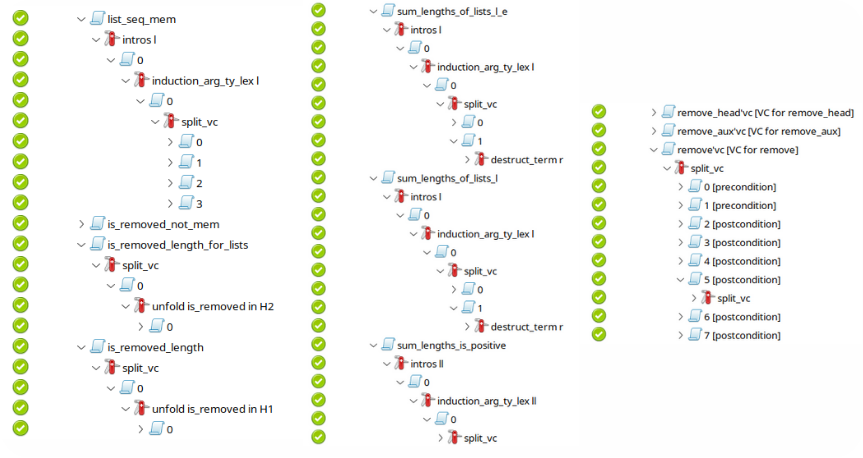
\includegraphics[width=0.5\textwidth]{images/removeWhy3IDE.png}
  \caption{\texttt{remove} proof in Why3 IDE}
  \label{fig:Why3Remove} 
\end{figure}

\subsection{Detect order inconsistencies in a list of lists}
\label{sec:detectOrderInconsistencies}
The function \texttt{merge} is the most complex function in the C3 linearization algorithm; this function receives a list of lists and returns a list where the order that each class has with each other respects in every list of the input.\\
To detect this, a precedence graph builds from the relations between the classes in the lists. For example, if we have the list of lists $((A, B, C),(C, D),(D, A))$, the graph in Fig.~\ref{fig:cyclicGraph} is built.
\begin{figure}[htbp]
  \centering
  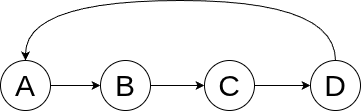
\includegraphics[width=0.25\textwidth]{images/cyclicGraph.png}
  \caption{Cyclic precedence graph}
  \label{fig:cyclicGraph}
\end{figure}
We can see that the graph is cyclic, and therefore, the order of the classes is inconsistent, and a linearization cannot be produced.
It must exist an element that for every list of a list, this element is not in the tail of the list, and it exists a head from a list that is equal to the element. % grammerly 
To detect the acyclicity of a graph, the following predicate was written:
\inputminted[firstline=64,lastline=80,fontsize=\small,linenos,xleftmargin=20pt]{ocaml}{../c3/cameleer/c3.ml}
This predicate ensures that for the graph to be acyclic, no path exists in the graph where the first class is the same as the last class.
The lemmas created that give use to this predicate are not proven in this project and are assumed by postconditions and preconditions of the \texttt{merge} and \texttt{c3\_linearization} functions.

\subsection{merge function}
The merge function is the core of the C3 linearization algorithm, and it is responsible for merging the lists of classes respecting the order of the classes in each list.
The function is defined as follows:
\inputminted[firstline=363,lastline=386,fontsize=\small,linenos,xleftmargin=20pt]{ocaml}{../c3/cameleer/c3.ml}
The function receives a list of lists, then for each head of the list is checked if it does not belong to any tail of the lists, 
if that condition is satisfied the head is removed from all the lists using the \texttt{remove} function, and the head is added to the result list.
\subsubsection{Termination}
The termination of the function (line 283) is ensured by the postcondition of the \texttt{remove} function, which states that the sum of the lengths of the lists decreases with each call, so if the variant is the sum of the lengths of the lists, then the function will terminate.
\subsubsection{Remove preconditions}
The preconditions of \texttt{remove}, states that for each call the element removed has to satisfy the condition previously described.
To prove that, is required that the list of lists have a precedence graph acyclic (line 366) and this ensures, has discussed in the section~\ref{sec:detectOrderInconsistencies}, 
that the element removed is not in the tail of any list. This is stated by the following unproved lemma:
\inputminted[firstline=198,lastline=203,fontsize=\small,linenos,xleftmargin=20pt]{ocaml}{../c3/cameleer/c3.ml}
\subsubsection{Main postconditions}
The two main postconditions of the \texttt{merge} function ensures that:
\begin{itemize}
  \item The result is a list of classes that respects the order of the classes in each list of the input (lines 369 to 376).
  \item All the result classes present in the final list must exist in one of the lists of the input (lines 377 to 384).
\end{itemize}
Even assuming the acyclicity lemmas, this proof has yet to be proven.
\subsubsection{Why3 IDE result}
In the image (Fig. \ref{fig:Why3Merge}), we can see the proof progress of the \texttt{merge} function in the Why3 IDE.
\begin{figure}[htbp]
  \centering
  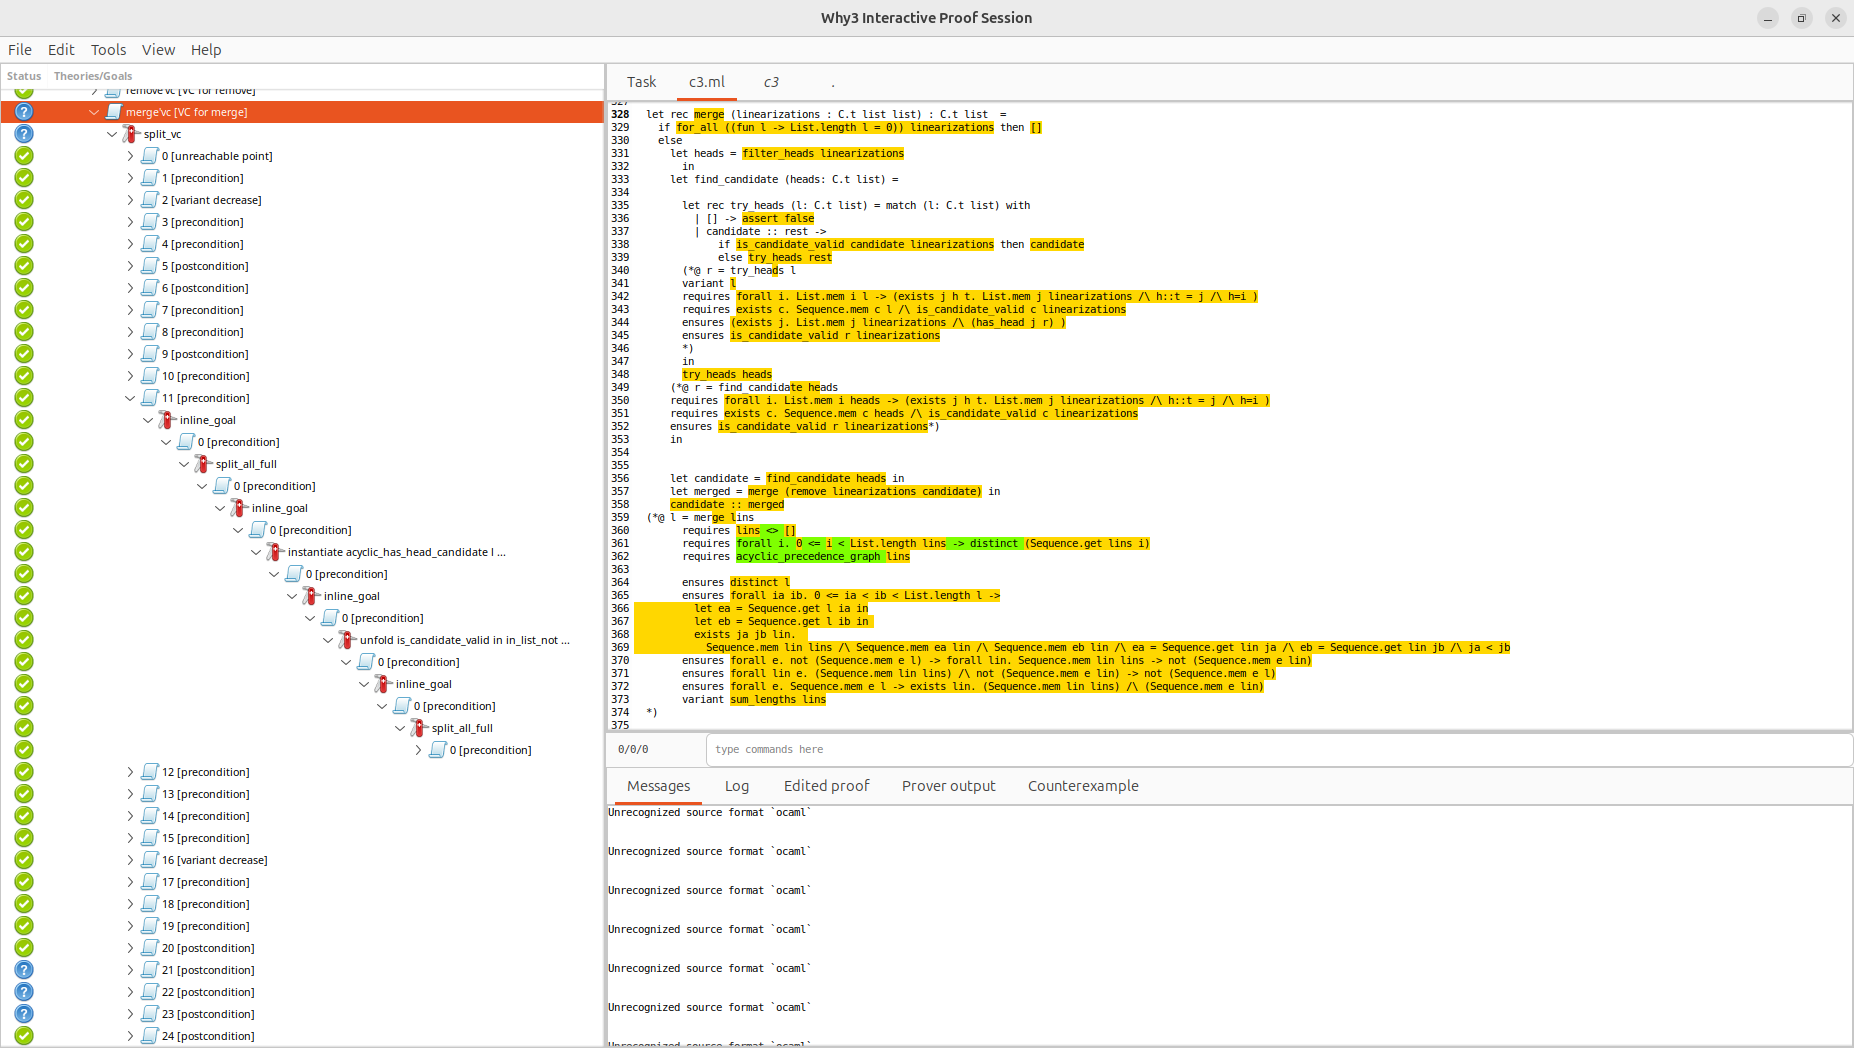
\includegraphics[width=0.8\textwidth]{images/Why3merge.png}
  \caption{\texttt{merge} proof in Why3 IDE}
  \label{fig:Why3Merge}
\end{figure}

\subsection{c3\_linearization function}
The \texttt{c3\_linearization} function differs from the original one to help the proof of termination, a new argument \texttt{universe} was added, which contains all the classes above in the hierarchy of the class.
In that way, every time the parents of a class are called in the function \texttt{linearize} (an auxiliary function of \texttt{c3\_linearization}), the class is removed from the universe, and the parents of the class are called with the universe as an argument.
This ensures that the hierarchy remains acyclic and because the universe is always decreasing at each loop, it can be passed as argument and termination is ensured.
Aside from the termination, the function is proved to be consistent with \texttt{merge} requirements.\\
Finally, all the goals and its verification can be seen in the image (Fig.~\ref{fig:Why3C3}).
\begin{figure}[htbp]
  \centering
  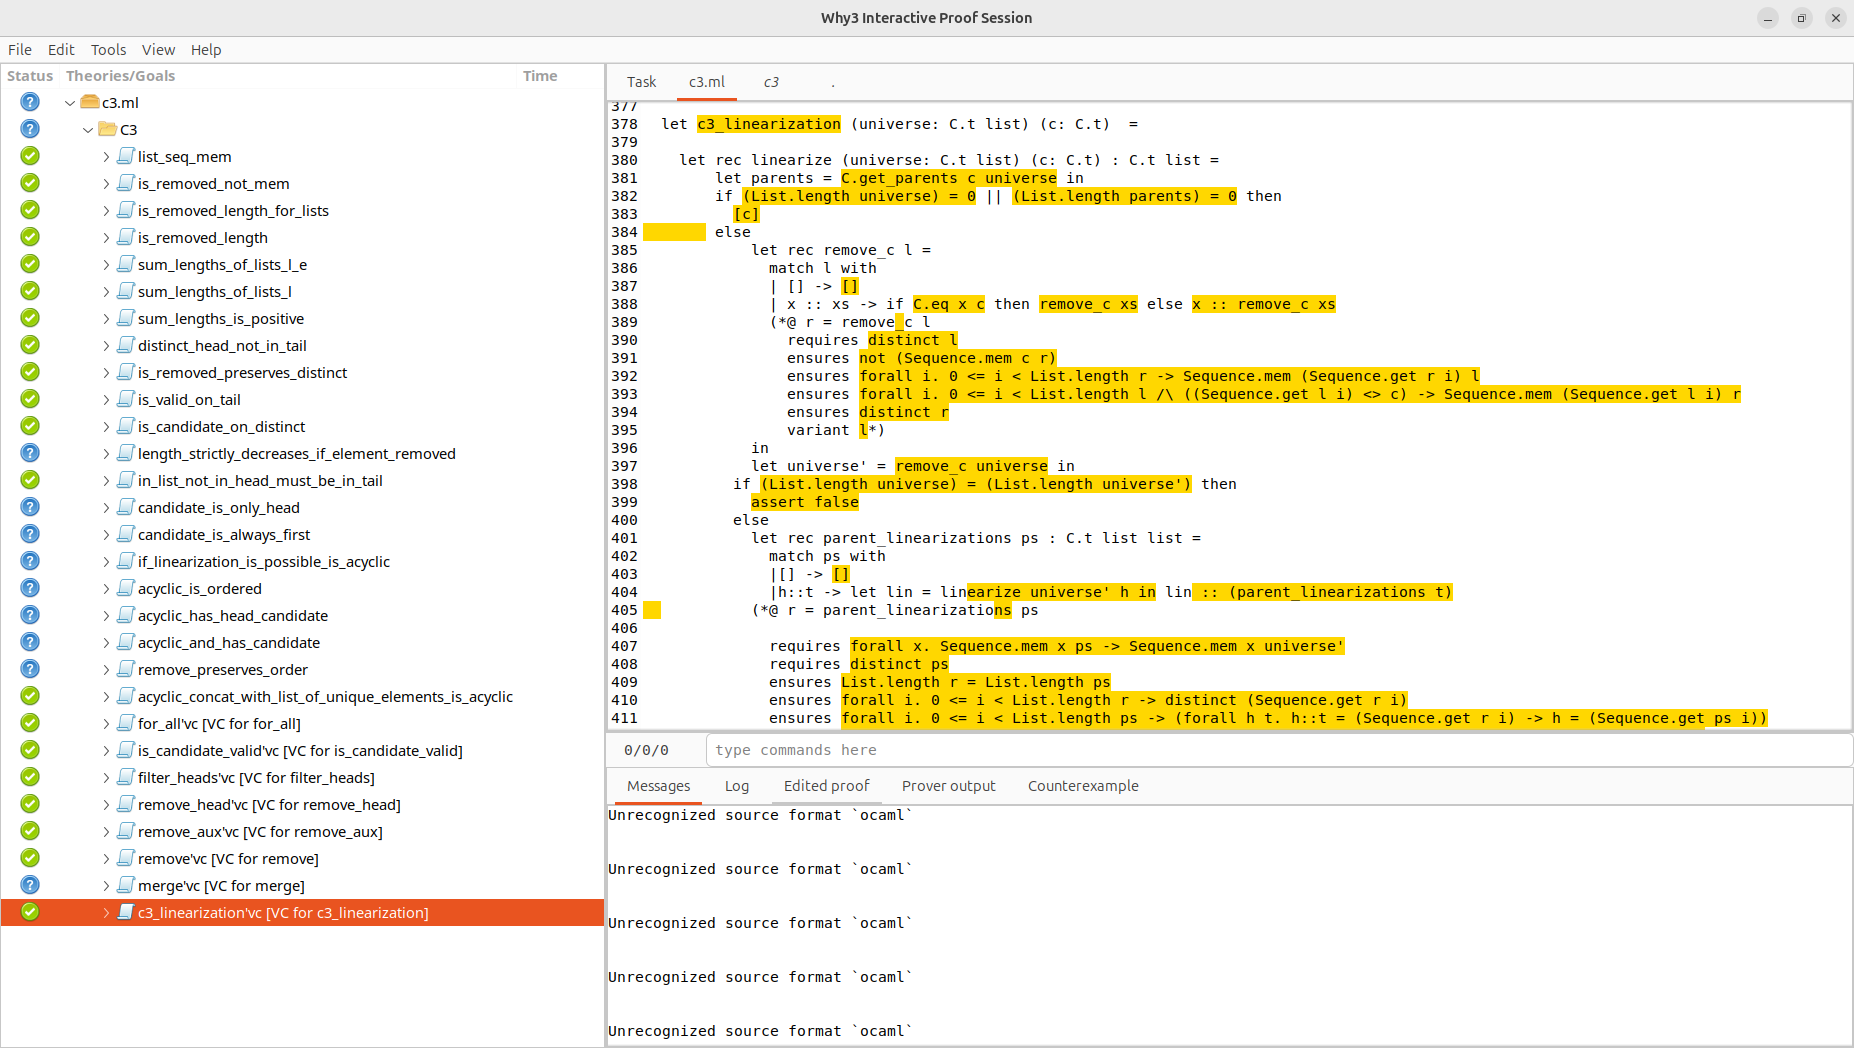
\includegraphics[width=0.8\textwidth]{images/Why3C3.png}
  \caption{All goals in Why3 IDE}
  \label{fig:Why3C3}
\end{figure}
\section{Related Work}
\label{sec:related-work}
While the C3 linearization algorithm is widely used in programming languages, 
there has been limited formal verification of its implementation.
Most existing works focus on informal descriptions or implementations in specific languages, such as Python\autocite{Python23Method} and Perl\autocite{MroMethodResolution}.
To our knowledge, no verified implementation of the C3 linearization algorithm exists in OCaml or any other language.\\
There is a formal specification of the algorithm\cite{reisSoliderSolidity2023}, but has a lot of errors and inconsistencies, nevertheless, it was a good starting point for our work.\\
There is a verified implementation\cite{castanhoAutoactiveVerificationGraph2022} of the OCaml library OCamlgraph\cite{filliatreBacktrackingOcamlgraph2025}, 
this verification uses a similar approach to detect acyclicity in graphs and uses the same technology as our work, Why3 and Cameleer.\\
To get extract the accurately C3 properties, we used the work of Florent Hivert and  others\autocite{hivertControllingC3Super2024}, which provides a detailed explanation of the C3 linearization algorithm and its properties.\\
To explore the effects of the multiple inheritance in programming languages, how it affects the MRO algorithms and how the diamond problem is resolved, we used the work of Fawzi Albalooshi and others\autocite{albalooshiComparativeStudyEffect2017}.

\section{Conclusion and Future work}
\label{sec:conclusion-future}
In this work, we addressed the need for a verified implementation of the C3 linearization algorithm, which is widely used in programming languages to resolve conflicts in multiple inheritance scenarios. 
We presented a mathematical formalization of the algorithm and initiated its verification using OCaml, Why3, and Cameleer. Our work proves termination and partially verifies the core components of the algorithm.

While the complete verification of the linearization process is still in progress, our contributions mark an important step toward a full proof of C3's correctness.

To complete the verification, we need to prove the acyclicity of the precedence graph. 
As discussed in Section~\ref{sec:related-work}, existing work on verifying acyclicity in Why3 and Cameleer provides a promising starting point for this task.

We also need to prove a lemma essential for the termination of the \texttt{merge} function, shown below:

\inputminted[firstline=151,lastline=158,fontsize=\small,linenos,xleftmargin=20pt]{ocaml}{../c3/cameleer/c3.ml}

We experimented with \texttt{Sequence.get} (access by index) instead of \texttt{Sequence.mem} 
(membership check) to support this proof, 
but this was not sufficient to establish the lemma or to prove the termination of the \texttt{merge} function.

Finally, we aim to verify the \texttt{c3\_linearization} function. This can be done by expressing as postconditions the 
properties defined in Section~\ref{subsec:PropertiesformalSpec}. To facilitate this, instead of using the \texttt{get\_parents} function (Section~\ref{subsec:CLASS}) with a universe as input, 
the algorithm should be passed a class hierarchy directly as an argument. This could follow the type signature \texttt{(t * t list) list}, where the \texttt{t list} represents the parents of class \texttt{t}.
\printbibliography

\end{document}
